\subsection{JavaServer Faces}

\par Segundo \citeonline{faria_java_ee_7_jsf_primefaces_cdi}, a tecnologia \textit{JavaServer Faces} - JSF\footnotemark[17] - foi definida pelo JCP (\textit{Java Community Process}), tornando-a um padrão de desenvolvimento, facilitando assim o trabalho dos desenvolvedores de software.

\footnotetext[17]{JSF: \textit{JavaServer Faces} - Framework que permite desenvolver páginas \textit{web} para aplicações desenvolvidas em Java.}

\par \citeonline{bergsten_javaserver_faces} afirma que o JSF é um \textit{framework server-side} baseado em componentes \textit{web}, cuja principal função é abstrair os detalhes de manipulação dos eventos e organização dos componentes na página \textit{web}. Por meio dele é possível desenvolver páginas mais sofisticadas de forma simples, abstraindo inclusive, o tratamento de requisições e respostas. Isto permite ao desenvolvedor focar-se no \textit{back-end} da aplicação, ou seja, na lógica, e não se preocupar com detalhes a respeito de requisições e respostas HTTP e como obter as informações recebidas e/ou enviadas através deste protocolo.

\par De acordo com \citeonline{oracle_javaserver_faces_technology_overview}, o JSF é de fácil aprendizado e utilização, pois possui sua arquitetura claramente definida, sendo dividida entre a lógica da aplicação e apresentação. Esta divisão é possível pois ele utiliza o padrão de projeto \textit{Model-View-Controller} - MVC\footnotemark[18] -, tornando-o um importante \textit{framework} para desenvolvimento de aplicações utilizando a plataforma Java \textit{Web} e com alta demanda no mercado.

\footnotetext[18]{MVC: \textit{Model-View-Controller} - \textit{Design pattern}.}

%BANCA_QUALIFICACAO. Comentado este parágrafo, porém o mesmo retornará para a banca de qualificação
\par Segundo \citeonline{gamma_helm_johnson_vlissides_design_patterns_elements_reusable_object_oriented_software}, o padrão de projeto MVC é dividido em três partes. O \textit{Model} é a lógica da aplicação, a \textit{View} é camada de apresentação e por último o \textit{Controller} é responsável por definir a interface entre a lógica e a apresentação. Portanto, todo tipo de requisição ou resposta deve ser obrigatoriamente enviada ao \textit{Controller}, que, por sua vez encaminhará para a camada de visão ou de lógica. A figura 7 demonstra um exemplo do modelo MVC utilizando o JSF.

% Imagem do modelo MVC usando JSF - VOLTAR PARA A BANCA DE QUALIFICACAO
\begin{figure}[h!]
	\centerline{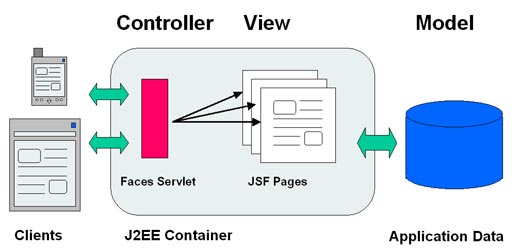
\includegraphics[scale=0.5]{./imagens/jsf_using_mvc.jpg}}
	\caption[Imagem de demonstração do Modelo MVC]
	{Imagem de demonstração do Modelo MVC \textbf{Fonte:} http://www.javabeat.net/jsf-2/}
	\label{fig:exemplo1}
\end{figure}

%BANCA_QUALIFICACAO. Comentado este parágrafo, porém o mesmo retornará para a banca de qualificação
\par Ao utilizar o JSF, toda e qualquer interação que o usuário realizar com a aplicação será executada por um \textit{servlet} chamado \textit{Faces Servlet}. Ela é a responsável por receber tais requisições da camada de visão e redirecioná-las à lógica da aplicação e, posteriormente, enviar a resposta ao usuário \cite{faria_java_ee_7_jsf_primefaces_cdi}.

\par Por possuir as vantagens descritas acima e possuir uma simples configuração, além de ser um \textit{framework cross-browser\footnotemark[19]}, este \textit{framework} foi escolhido para auxiliar no desenvolvimento das páginas \textit{web} deste projeto.

\footnotetext[19]{\textit{Cross-Browser} - Compatibilidade com todos os tipos de dispositivos e navegadores}
